\documentclass[a4paper,11pt, oneside]{article}  % document class
\usepackage{geometry}
\geometry{
inner=20mm,
outer=18mm,
top=25mm,
bottom=23mm %
%  heightrounded,
%  marginparwidth=50pt,
%  marginparsep=17pt,
%  headsep=20pt
}
\usepackage[english]{babel}
\usepackage{hyperref}
%pacchetto
\usepackage{import, multicol,lipsum}  % package
\setlength{\columnsep}{1cm}

\usepackage[utf8]{inputenc} % accenti facili
\usepackage[T1]{fontenc}
\usepackage{subcaption}
\usepackage{pifont}
\usepackage{url}
\hypersetup{
colorlinks=true,
linkcolor=blue,
filecolor=magenta,      
urlcolor=blue
}
\usepackage{graphicx, color, blindtext}
\usepackage{textcomp, makeidx, times}
\usepackage{amsthm, amsmath, amssymb, amsfonts, mathtools} % math
\usepackage[mathscr]{eucal}		
\usepackage[nottoc]{tocbibind} 
\usepackage{pgfplots, parskip}
\usepackage{afterpage, ifthen}
\usepackage{enumitem}
\pgfplotsset{compat=newest}
\usepackage{graphicx} % immagini
\usepackage{wrapfig}
%\graphicspath{ {image/} } % path cartella delle immagini
\usepackage{tikz} %graph
\usetikzlibrary{arrows,automata}
\usetikzlibrary{automata,arrows,positioning,calc,matrix}
\usepackage[linesnumbered,ruled,vlined]{algorithm2e}
\usepackage{booktabs}
\usepackage{colortbl}
\usepackage{siunitx}
\usepackage{tabularx, tabu}
\usepackage{relsize}
\usepackage{makecell, caption, chngcntr}
\usepackage{bbm}
\usepackage{diffcoeff}
\RequirePackage{fix-cm}


%
%____________________________________________________________________________________________________________________________
%____________________________________________________________________________________________________________________________
%____________________________________________________________________________________________________________________________
%____________________________________________________________________________________________________________________________
% INIZIO
\begin{document}

\setcounter{secnumdepth}{2}
\pagestyle{plain} % stile pagina (header, numerazioni)

% \centerline {
\includegraphics[width=2cm]{logo.jpg}}
\begin{center}
	Università degli Studi di Torino - M.Sc.  in Stochastic and Data Science - A.Y.  2021/2022 \\
	\Large { Final project of Statistical Machine Learning (MAT0043)}
	\line(1,0){450}\\ 
	\vspace{0.4cm} 
	{ \huge \textbf{Gene selection for cancer type classification} }
	\vspace{0.1cm}
	\line(1,0){450} \\
\end{center}

%____________________________________________________________________________________________________________________________

The purpose of our project is to work on a high-dimensional genomics dataset and find a relatively small number of genes to predict the cancer type of a given tumorous cell. This is known as Genes Selection for Cancer Classification and it is in line with many up-to-date researches in applied medicine.  Our dataset contained $1.032$ cancerous cells and their knock-out probabilities, i.e.  the probabilities of stopping the growth of the tumor by inhibiting one of the $\sim 17.000$ studied genes.  We explore in detail three Features Selection algorithms,  namely Random Forests (RF) combined with Feature Importance,  Lasso-SVM and Neural Networks (NN) combined with Olden,  and find that the possibility of classifying the cancer type from an extremely small set of genes mainly depends on the cancer type itself.  


\section{Introduction}
Cancer is a complex illness characterized by the uncontrolled growth of abnormal cells anywhere in the body.  In recent years,  medicine has made a great step forward in finding new and efficient therapies for different diseases,  including cancer.  Thanks to numerous advances in technology,  collecting huge amount of data is no longer an issue,  so that one can exploit this information to define personalized treatments for patients.  In this regards,  the DepMap project\footnote{DepMap Portal: \url{https://depmap.org/portal/} } and,  in particular,  the Achilles project\footnote{Achilles Project: \url{https://depmap.org/portal/achilles/} } aim to use genome-wide screens to collect data regarding mutations of cancerous cells,  identify essential genes and report vulnerabilities across hundreds of human tumours. 

Many researchers are currently using DepMap datasets to identify a small number of genes which are responsible of cancer growth\footnote{Background material: \url{https://depmap.org/portal/publications/}}. This procedure is often driven by medical knowledge,  which we do not possess,  together with some rough measures of importance.  Being Maths students, we instead base our research on statistical models and on the hypothesis that "if a given classifier is able to distinguish different types of cancer,  then the most relevant genes are the most important features for that classifier" (the meaning of \textit{important} will be clarified later).  Of course,  selecting few truly significant genes has outstanding implications in the medical field: building faster diagnosis tools and synthesizing less toxic drugs are only two examples. 


\section{Dataset}
We use two public datasets from the DepMap Public 21Q3 database,  released on August 2021\footnote{Download dataset from DepMap:  \url{https://depmap.org/portal/download/}}:
\begin{itemize}
	\item \textit{CRISPR\_gene\_dependency.csv}, containing $1.032$ cancer cells and their $17.393$ gene scoring results;
	\item \textit{sample\_info.csv}, containing cell lines information,  such as primary disease and sample collection site.
\end{itemize}
Data were collected from real patients and successively processed,  so that element $(i, j)$ of this $(1.032 \times 17.393)$-data frame is the probability that knocking out gene $j$ has a real depletion effect on the $i$-th cell.  Each example has a label (reported in the \textit{sample\_info.csv} and that is why we need this second dataset) which indicates the tumour.  We group the various cancer types in 10 classes according to common medical knowledge\footnote{Cancer types grouped by body location: \url{https://www.cancer.gov/types/by-body-location}} and obtain the groupings reported in Figure \ref{fig1}. 

\begin{wrapfigure}{r}{0.7\textwidth}
	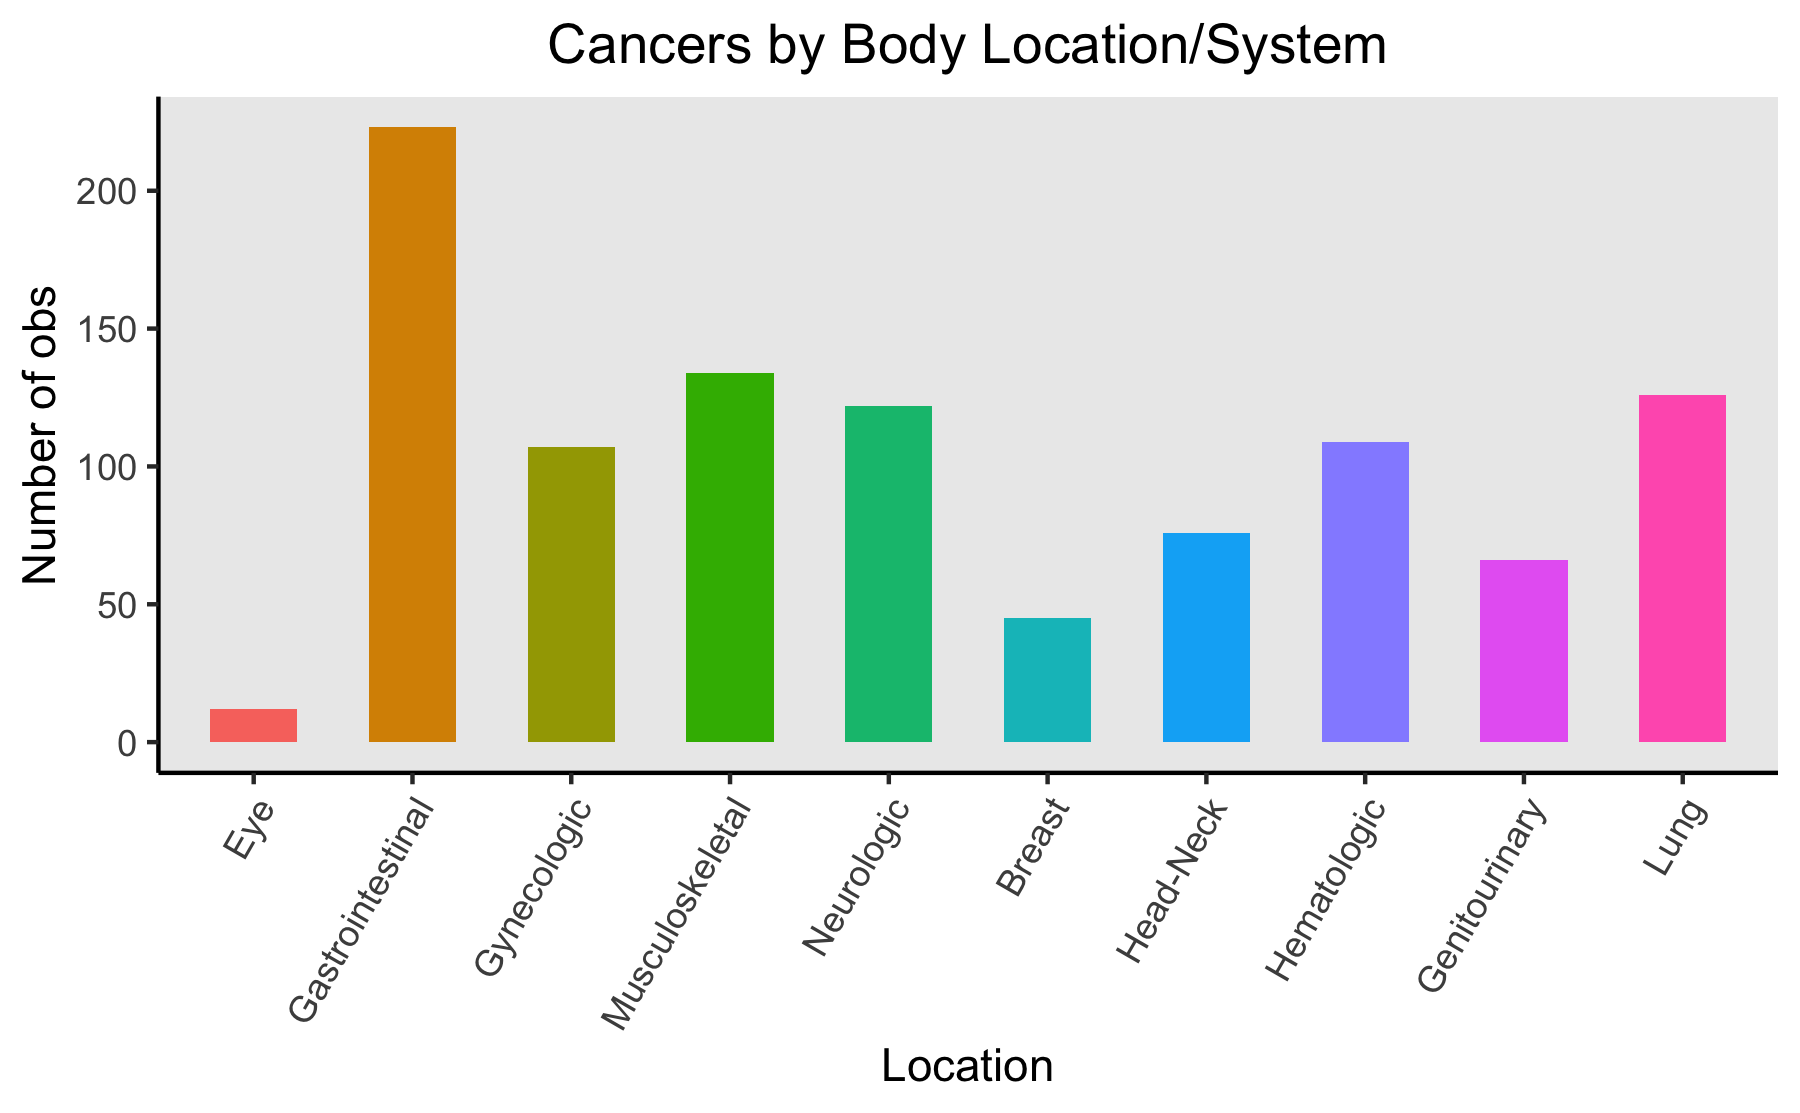
\includegraphics[width=0.7\textwidth]{plot1.png}
	\captionof{figure}{Cancer classes}\label{fig1}
\end{wrapfigure}
"Eye" is the smallest class as there are only $16$ observations, whereas "Gastrointestinal" is the largest one and it comprehends $7$ kinds of cancer,  making this group quite heterogeneous. 

We investigate two Binary classification problems,  Blood vs Rest and Lung vs Rest, and the Multiclass problem. \\
We choose "Lung" because it is the most numerous group and it is composed by lung cancer cells only.  The choice of "Blood" is instead driven by some underlying biological knowledge: Blood cancer is quite different from other tumours because
\begin{itemize}
	\item Leukemia, Lymphoma and Myeloma are the main kinds of cancer but they all affect white blood cells;
	\item blood is in the whole body, and so the illness is too.
\end{itemize} 

\section{Methods}
% Let us briefly illustrate the algorithms we used. 
\subsection{Random Forest}
We use Random Forest (RF) as they frequently perform well on correlated high-dimensional data and Variable Importance to identify the most relevant features. This measure is calculated in three steps.  

\begin{wrapfigure}{l}{0.318\textwidth}
	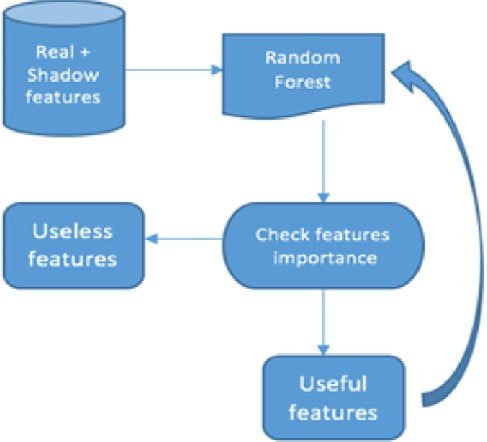
\includegraphics[width=0.318\textwidth]{Boruta-Algorithm.jpg}
	\captionof{figure}{Boruta Algorithm}\label{fig2}
\end{wrapfigure}
First, prediction accuracy is measured on the out-of-bag samples. Then, values of the variable are randomly shuffled, keeping all other variables the same.  Finally, the decrease in prediction accuracy is measured on the shuffled data and the mean decrease in accuracy across all trees is reported.  Intuitively, random shuffling means that, on average, the shuffled variable has no predictive power. 

Hence, Variable Importance measures how much accuracy decreases because of variables removals. We can exploit it in two different ways:
\begin{itemize}
	\item \textit{Cross-validation}: we perform a 5-fold Cross-validation on the model, average the importance values and select the top most important features;
	\item \textit{Boruta algorithm}\footnote{Boruta algorithm: \url{https://www.researchgate.net/publication/220443685_Boruta_-_A_System_for_Feature_Selection}}: Boruta repeatedly computes features importance and then performs statistical tests to screen out irrelevant predictors. Simple scheme is presented in Figure \ref{fig2}.
\end{itemize} 
\newpage

\subsection{SVM-Lasso}
Support vector machines (SVM) are based on the idea of finding a hyperplane that best separates classes. We combine this method with the classical Lasso penalty, thus the objective function to be minimized becomes:
\begin{equation*}
\dfrac{1}{n} \sum_{i=1}^n hingeLoss(y_i(x_i w + t)) + \lambda ||w||_1  \qquad	\text{where} \qquad  hingeLoss(z) = max\{0, 1-z\}
\end{equation*}
The parameter $\lambda$ is chosen via cross-validation. Thanks to Lasso penalty, we obtain sparsity in predictors: some $w_i$ are shrunken all the way to zero while the others identify important features. 

\subsection{Neural Networks}
Neural Networks (NN) are efficient models to capture non-linear relationships between predictors and target variables.

\begin{wrapfigure}{l}{0.45\textwidth}
	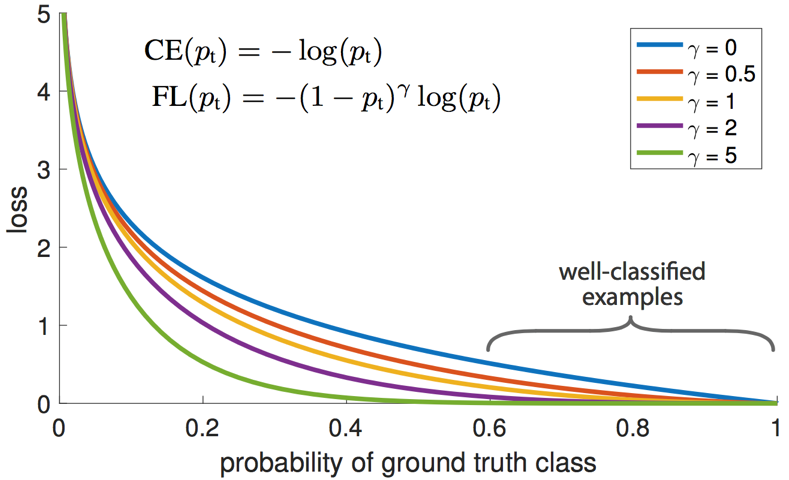
\includegraphics[width=0.45\textwidth]{nn-focal-loss.png}
	\captionof{figure}{Cross Entropy and Focal Loss}\label{fig3}
\end{wrapfigure}
In this context, we train NNs with two hidden layers of width $400/500$ and $300$. We choose \textit{ReLU} as activation function for the hidden layer, \textit{sigmoid} and \textit{softmax} for the output layer for the  Binary and Multiclass respectively.

Since the Binary problems are a little unbalanced, we try both the usual \textit{Cross Entropy} loss function and the \textit{Focal Loss}, defined as 
\begin{equation*}
FL(z) = - \alpha (1 - z)^{\gamma} \log{z} \text{, with }z \in [0,1]  \text{ and } \alpha,  \gamma \geq 0
\end{equation*}
Special cases of these functions are drawn in Figure \ref{fig3}. \\
In particular, \textit{Focal Loss} can be extended and used in Multiclass classification tasks\footnote{Focal Loss: \url{https://arxiv.org/pdf/1708.02002.pdf}}.

Once our NNs have been fitted, we rank variables according to the Olden Importance measure\footnote{Olden Importance: \url{https://depts.washington.edu/oldenlab/wordpress/wp-content/uploads/2013/03/EcologicalModelling_2004.pdf}},  select a few hundreds of them and train a reduced version of the classifiers. 

\subsection{Methodology}
Notice that NN and RF are Wrapper Feature Selection methods and so that our methodology is characterized by:
\begin{enumerate}
	\item fitting the model using all the features;
	\item identifying the most important variables based on some measure of importance; 
	\item using those genes to fit a reduced version of the classifier and find out its performance.
\end{enumerate} 
Clearly, each procedure involves fitting a model twice: the all-features version and the reduced one.  We are then forced to split the dataset into two further chunks, which will be referred as D1 and D2. In fact, this is crucial to ensure independence of the two models and remove any sort of correlation.

In the case of SVM-Lasso, which is an Embedded Feature Selection method, the Lasso penalty already provides variable selection. Thus, important genes are the ones associated with non-zero weights and, consequently, we do not need to split the dataset. 

\section{Results}
We now present the outcomes obtained by fitting the models discussed above. \\
These results are expressed in terms of average recall, i.e. $\frac{1}{k} \sum\limits_{i = 0 }^k r_i$, where $r_i$ is the rate of correct predictions for class $i$ and $k$ is the total number of classes. We prefer not to rely on the usual accuracy measure,  which is defined as \textit{total correct prediction / number of observations}, because it conveys a misleading message. For example,  we reach $90\%$ accuracy in Lung vs Rest classification but our classifier completely disregards Lung instances (which are indeed $10\%$ of the total) as it always predicts the Rest class.  

\subsection{Binary classifications: Blood vs Rest}
We obtain remarkable results in Blood vs Rest classification. We initially fit a \textbf{Random Forest} (RF) classifier on D1. Even though Blood cancer observations are only the $11\%$ of the total,  we do not need any adjustment for the minority class.  Indeed, thanks to proper tuning on trees parameters and a correction on class weights, we reach $98\%$ of average recall,  see Table \ref{table:big_models}. For the sake of completeness, we build also a RF with Cost-Complexity Pruning and we find the same result. We then focus on feature selection using both RF Variable Importance and the Boruta algorithm. As shown in Table \ref{table:selected variables},  Boruta individuates a higher number of important features than our manual method and,  in particular,  they agree on $84$ genes. We train now two RFs on D2, one for each set of selected features. Besides weighting classes, no further parameters are specified and nevertheless both RF classifiers predict correctly $6$ tumour cells out of $7$,  with an average recall of $93\%$.

As a second model, we explore \textbf{SVM-Lasso}. In this case $108$ important genes are selected and the average recall is $97\%$, as reported in Table \ref{table:reduced_models}. Furthermore, $12$ important features are shared with the RF model, which made us think those genes are important in the medical field.

Furthermore, \textbf{Neural Network} (NN) classifier achieves outstanding performance as well.  In this case,  instead of tuning the NN parameters to take into account the Blood minority class,  we decide to fit $50$ NNs on $50$ different undersampled versions of D1 and then take the mean class probability to make predictions. Such datasets are constructed by retaining all the Blood observations and randomly picking as many Non-Blood observations.  Having reached a high average recall, namely $99.1\%$,  we select the most important genes according to Olden's importance (we have to use Vultr cloud computing\footnote{Vultr cloud computing: \url{https://www.vultr.com}} because of high computational costs). Here we pick slightly more features than RF and fit a "vanilla" neural network with one single hidden layer on D2.  As a result, we obtain an average recall of $99.3\%$ and all Blood cancer cells are correctly classified. 
\medskip

\subsection{Binary classifications: Lung vs Rest}
Unfortunately,  we could not build a proper model for Lung vs Rest.  Even after a tuning of the tree parameters,  the \textbf{RF} is not able to detect the minority class.  Thanks to SMOTE, we adjust the frequency of those observations from $11\%$ to $50\%$ and now the refitted RF gives us a slightly better result: at least one third of Lung cancer cells is correctly predicted.  Similar results are achieved with Minimal Cost-Complexity Pruning. Poorly outcomes have been found for \textbf{NNs} as well, even using the \textit{Focal Loss}, and for \textbf{SVM-Lasso}. We report all average recalls in Table \ref{table:big_models}. Since all these models are not good enough in classifying Lung cancer, we feel that selecting the most important features is pointless and incorrect in terms of real applications. Therefore, no reduced model will be fitted.
\medskip

\subsection{Multiclass classification}
When working with the Multiclass problem, we decide to remove the group "Eye" as it is too small and heterogeneous, hence extremely difficult to be detected by the classifier. 
\medskip

Let us consider the \textbf{RF} classifier. We initially fit it with balanced weights for classes: the results are satisfying in terms of average recall, but for the Gastrointestinal class, which is the most heterogeneous group. By means of 5-fold Cross validation, we extract the most important features and look at their relative importance. A new RF is then fitted on D2 with the first $465$ genes. Here, the manual tuning of the class weights limits the effect of Gastrointestinal and gives better results.  At last, we also exploit Boruta algorithm and we find fewer important variables than with Cross-validation,  as one can see in Table \ref{table:selected variables},  but the two RFs models achieve a similar average recall.

Let us study \textbf{SVM-Lasso} as a second model.  Although it is particularly suited for binary classification tasks, we extend it to the Multiclass problem by using the so-called OVO (One vs One) approach. In other words, we take every possible combination of two classes and we construct an SVM-Lasso model for each pair. We then end up with $ \binom{9}{2} = 36$ models so that predictions are determined by seeing which class wins more "duels". Again,  being an embedded model, feature selection is already achieved by fitting the model once.  Results are displayed in Tables \ref{table:reduced_models} and \ref{table:selected variables}. Notice that the high number of selected features depends on the fact that there are 36 models.  

Finally, \textbf{NN}. We fit three different NNs: one using the \textit{Cross Entropy} and the other two with \textit{Focal Loss}, but changing the $\alpha$ parameter w.r.t. class percentages. In particular, these last models are slightly more accurate. We take the best one to rank variables according to Olden Importance measure.  Here, we are forced to retain more genes than in the binary classification task simply because separating $9$ classes requires more information. The average recall of the new classifier is shown in Table \ref{table:reduced_models}.
\bigskip

\begin{minipage}[c]{0.4\textwidth}
	\centering
	\begin{tabular}{c c c}
		\hline\hline
		Task & RF & NN \\ [0.5ex] % inserts table %heading
		\hline
		Blood & 0.991  & 0.986 \\
		Lung & 0.649  & 0.627 \\
		Multiclass & 0.655 & 0.702 \\ [1ex]
		\hline
	\end{tabular}
	\captionof{table}{Average recall, all-features models}
	\label{table:big_models}
\end{minipage}
\hspace{0.3cm}
\begin{minipage}[c]{0.5\textwidth}
	\centering
	\begin{tabular}{c c c c c}
		\hline\hline
		Task & RF-Cv & RF-Boruta & SVM-Lasso & NN-Olden \\ [0.5ex]
		\hline
		Blood & 0.929 & 0.929 & 0.984 & 0.993 \\
		Multiclass & 0.525 & 0.489 & 0.603 & 0.494 \\ [1ex]
		\hline
	\end{tabular}
	\captionof{table}{Average recall, reduced models}
	\label{table:reduced_models}
\end{minipage}
\bigskip

\begin{table}[h!]
	\centering
	\begin{tabular}{c c c c c}
		\hline\hline
		Task & RF-Cv &  RF-Boruta & SVM-Lasso & NN-Olden \\ [0.5ex] 
		\hline
		Blood & 109 & 118 & 108 & 300 \\
		Multiclass & 645 &  41 & 10.001 & 1.700 \\ [1ex]
		\hline
	\end{tabular}
	\caption{Selected variables}
	\label{table:selected variables}
\end{table}

\section{Conclusion and future works}
We can conclude that classifying cancer type from an extremely small set of genes heavy relies on the cancer type itself: our classifiers are able to distinguish Blood cancer almost perfectly but fail on Lung Cancer.  Note that this is also supported by the results of the multiclass task. Here, the significant decrease of the average recall can be attributed to bad-behaved classes such as Lung (again!) and Gastrointestinal. Thus, a future study might focus on these classes and find models which are able to recognize them.  From a more general perspective,  we admit that we do not have any hint about the meaning of selected genes and what is their role in the DNA.  Hence, it could be interesting to involve Med students into a similar project and base our work on a more solid medical knowledge.  

As stated in the Introduction, this project could have several implications and make a positive impact on people's lives. For example, if one were able to achieve high recalls on every class, then these results can be used to synthesize less toxic drugs that target only specific genes or to build fast diagnostic tools. In this regard, one should also include the class "No Cancer" as a control sample. Indeed, the DepMap project provides data of tumorous cells only, but it could be of interest repeating the study with healthy cells too.  
\end{document}